\documentclass{TDP005mall}
\usepackage{graphicx}
\usepackage[normalem]{ulem}
\newcommand{\version}{Version 1.0}
\author{Agnes Hallberg, \url{agnha531@student.liu.se}\\
  Eric Jönsson, \url{erijo137@student.liu.se}}
\title{Kodgranskning}
\date{2018-12-11}
\rhead{Agnes Hallberg\\
  Eric Jönsson\\}
\begin{document}
\projectpage

\section*{Revisionshistorik}
\begin{table}[!h]
\begin{tabularx}{\linewidth}{|l|X|l|}
\hline
Ver. & Revisionsbeskrivning & Datum \\\hline
1.0 & Första utkast  & 18-12-11 \\\hline
\end{tabularx}
\end{table}

\section{Inledning}
I detta dokument kommer processen sam resultatet av kodgranskningen behandlas.

På grund av sjukdom skedde inget fysiskt möte, utan koden delades mellan grupperna via GitLab. Varje grupp granskade den motsatta gruppens kod och överlämnade ett dokument med kommentarer. Överlämningen av kod skedde i slutet av arbetsdagen måndagen den 10:e december. Granskningen samt överlämningen av respons skedde under tisdagen den 11:e december.

\section{Vår granskning}
Vi lade stort fokus på att granska den objektorienterade designen. Vi blev imponerade av deras arbete. Koden hade bra intern struktur och en genomtänkt klasshierarki. Det var väldigt lågt beroende mellan klasserna tack vare deras välkonstruerade PlayState. Vidare var de konsekventa i sin namngivning och använde const på korrekt sätt.

Ett problem vi stötte på tidigt under granskningen var deras kodstruktur. De hade valt att ha varje klass i en egen fil. Det var lätt att få en överblick av vilka klasser som existerade, men att förstå klasshierarkin blev ett visst arbete då varje fil var tvungen att besökas och granskas för att förstå sambanden mellan klasserna. Vi föreslog att dela upp klasserna i färre filer; ha basklassen samt alla klasser som ärver av den i en headerfil. Detta hade lett till fyra headerfiler istället för de nuvarande tio.

Nedan kan en simpel illustration av klasshierakin ses som den tolkats av vederbörande.
\begin{figure}[h!]
  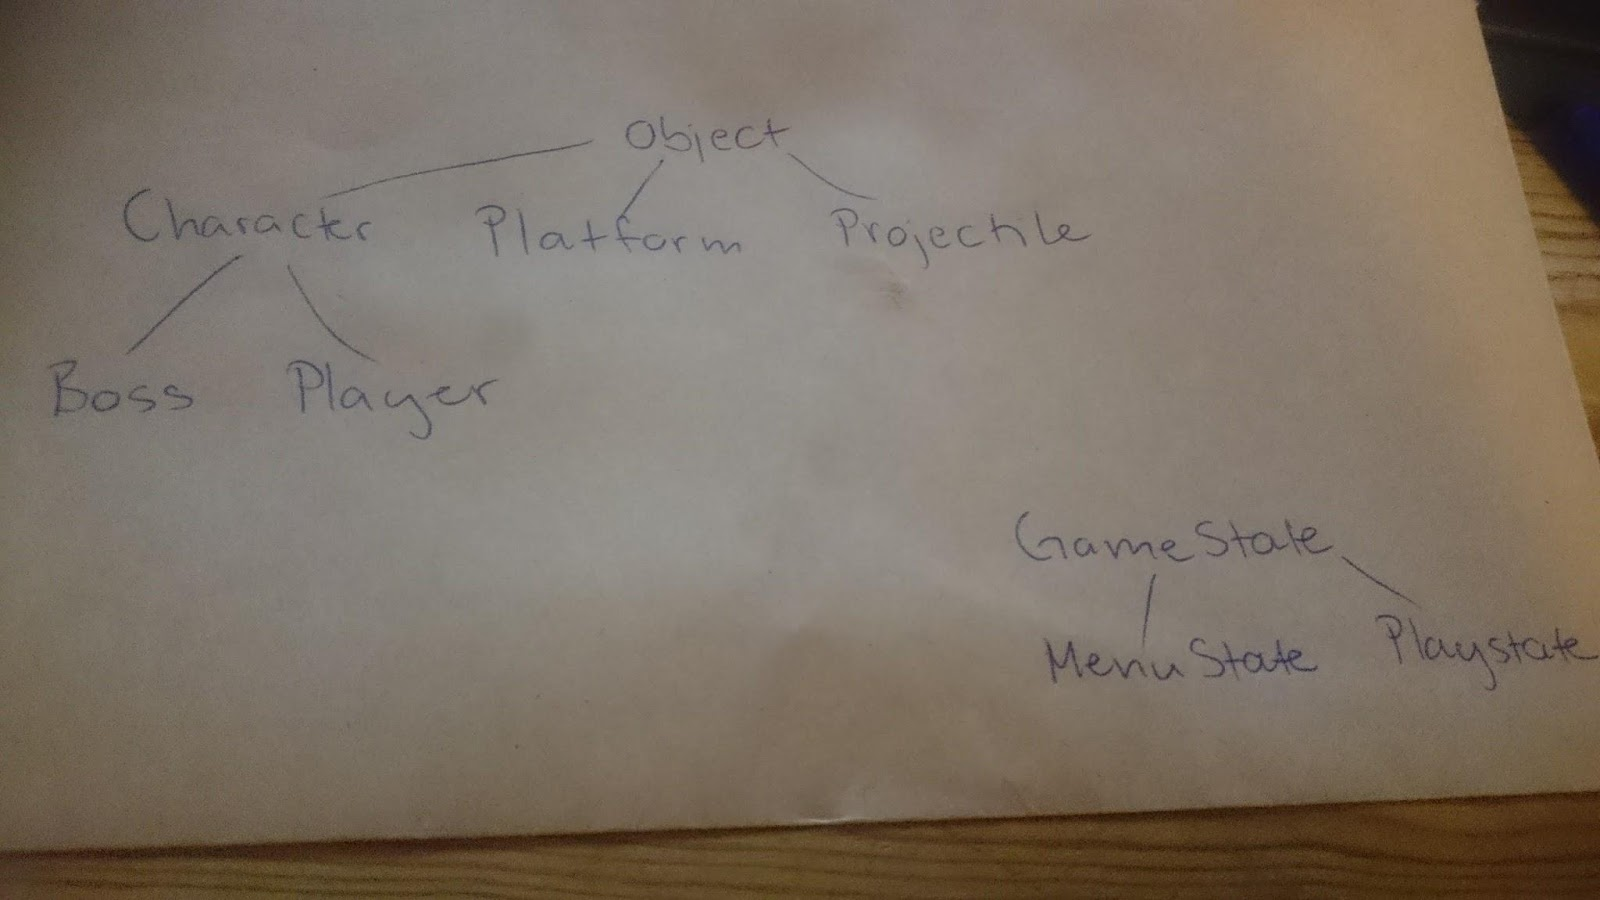
\includegraphics[width=0.75\linewidth]{klasser.jpg}
  \caption{Illustration av klasshierarki.}
\end{figure}

En annan sak vi reflekterade över var problematiken i att enkelt implementera fler typer av projektiler och plattformar.

Figur 1 ovan visar hur Boss och Player ärver från en egen klass, Character. Implementationen av en ny Character görs därmed väldigt enkelt; basmallen är redan skapad. Platform och Projectile saknar denna basklass och implementationen av till exempel en ny Projectile görs svårare på grund av detta. Vi förstår designvalet i och med projektets omfattning, men yrkade ändå på att det är viktigt att ha detta i åtanke vid framtida åtaganden.

En sista synpunkt vi hade var att SFML:s standardbibliotek hade kunnat utnyttjats bättre. Object hade kunnat ärva från SFML:s Sprite för att lätt kunna komma åt funktioner som move(), getPosition(), med mera. Vid tillfället för kodgranskning hade de implementerat dessa funktioner själva.

\section{Deras granskning}
De synpunkter vi fick var att vi kunde dela upp vår kod i fler filer, att vi kunde använda mer const samt att få ner de rader kod som krävs för att skapa ett nytt objekt. De påpekade även att de ville se mer av logiken ligga i PlayState och inte i main.

Vi fick beröm för vår flitiga användning av SFML:s standardbibliotek samt för vår klasshierarki. Vidare tyckte de även vår namngivning var god.

\section{Slutledning}
Det är svårt att säga hur mycket deras feedback kommer påverka vårt arbete då vi fortfarande har en del att implementera. Vi har skapat “slarvkod” i framförallt main-funktionen för att testa varje ny implementation. Det nuvarande skicket av vår kod är inte en rättvis representation av hur vi föreställer oss slutprodukten.

Det vi har reflekterat över är om det finns bättre strategier för att producera “renare” kod från start. Vi kunde ha implementerat de övergripande spelfunktionerna först för att enkelt kunna testa de senare implementationerna och kapat behovet av “skräpkoden” redan från början.

Dock kändes det mer övergripligt att börja med de små delarna först, som att få spelaren att flytta sig, än att skapa olika GameStates att växla mellan till exempel. 

Vi kommer ha en ordentlig städning av koden när vi är nöjda med de kodlösningarna vi producerat.

\end{document}
